% \setcounter{section}{-1}

\chapter{热力学基本定律}

%\section*{宏观}

热力学研究的对象是由大量微观粒子(分子或其他粒子)组成的宏观物质系统。
与系统发生相互作用的其它物体称为外界。
% 由于宏观测量的粗糙性,系统的宏观描述与大多数原子坐标不直接相关。热力学只关心大量原子坐标的平均后的宏观量。

\begin{definition}
	{热力学系统的分类}{thermodynamical system}
	根据系统与外界相互作用的情况,可以将系统分为:
	\begin{itemize}
		\item 孤立系统(isolated system):与外界既没有物质交换也没有能量交换;
		\item 封闭系统(closed system):与外界没有物质交换,但有能量交换;
		\item 开放系统(open system):与外界既有物质交换,又有能量交换。
	\end{itemize}
\end{definition}

\begin{remark}
	由于物质的普遍联系和相互作用,孤立系统的概念实际上只是一个理想的极限概念。
	% 实际情况是,当系统与外界的相互作用十分微弱,交换的粒子数远小于系统本身的粒子数、相互作用的能量远小于系统本身的能量,我们就把系统看作孤立系统。
	% 以后我们会看到,这一概念在热力学和统计物理中是十分重要和有用的。有关开系的问题将在第三章以后讨论,目前暂不考虑。
	% 有的作者将孤立系定义为与其它物体完全没有相互作用的系统,有的作者将孤立系定义为与其它物体既没有物质、也没有能量交换的系统。我们采用后一定义。它既包括与其它物体完全没有相互作用,也包括处在恒定外场(重力场、静电场、静磁场等)的情形。在与其它物体没有物质和能量交换的情形下,撤去系统的某种内部约束,不破坏系统的孤立性。我们以后会遇到这种情形。
\end{remark}

% 宏观物质可以用很少的量表征。这种特性源于:
% \textit{宏观测量与原子时间尺度相比极其缓慢,与原子空间尺度相比十分粗糙。}
% 宏观体系忽略了系统内部每个粒子的具体运动,正如Anderson所说:\textbf{\textit{More is different.}}
% 而热力学便是\textit{唯象}地描述多粒子行为的宏观理论。

\section{热力学第零定律:平衡态}

\begin{definition}
	{平衡态}{equilibrium state}
	经验指出,一个孤立系统,不论其初态如何复杂,经过足够长的时间后,系统的所有宏观性质在长时间内不发生任何变化。
	称为平衡态(equilibrium state)。
\end{definition}

% \begin{remark}
% 	系统由初始状态达到平衡态所需的特征时间称为弛豫时间(relaxation time)。弛豫时间可以很短也可以很长。以通常条件下的气体为例。通过分子的频繁碰撞,气体在10⁻¹⁰s左右就可以在小区域内建立局域平衡,而整个气体的平衡则要通过诸如扩散、热传导等过程才能实现。浓度的均匀化在气体中可能需要几分钟,在固体中则可能需要数小时、数星期甚至更长的时间。
% \end{remark}

\begin{remark}
	在平衡态之下,系统的宏观性质虽然不随时间改变,但组成系统的大量微观粒子仍处在不断的运动之中,只是这些微观粒子运动的统计平均效果不变而已。
	% 因此热力学的平衡态是一种动的平衡,常称为热动平衡。
	% 系统宏观物理量的数值仍会发生或大或小的涨落(fluctuation),这种涨落在适当的条件下可以观察到。不过,对于宏观的物质系统,在一般情况下涨落是极其微小可以忽略的。在热力学中我们将不考虑涨落,而认为平衡态下系统的宏观物理量具有确定的数值。
\end{remark}

\begin{remark}
	% 前面给出了孤立系统平衡态的定义。
	平衡态的概念不限于孤立系统。
	对于非孤立系统,可以把系统与外界一起看作一个更大的孤立系统。
	非孤立系统的平衡态就等价于这个更大的孤立系统的平衡态。
	% 我们以后会看到,对于处在各种条件下的系统,热力学用相应的热力学函数作为判据判定系统是否处在平衡态,并导出存在相互作用的两个系统达到热动平衡的平衡条件。
\end{remark}

% 现在讨论如何描述一个热力学系统的平衡态。
% 前面已经说过,在平衡态之下,系统各种宏观物理量都具有确定值。
% 热力学系统所处的平衡态就是由其宏观物理量的数值确定的。由于宏观量之间的内在联系,表现为数学上存在一定的函数关系,这些宏观量不可能全部独立地改变。
% 我们可以根据问题的性质和考虑的方便选择其中几个宏观量作为自变量。
% 这些自变量本身可以独立地改变,我们所研究的系统的其它宏观量又都可以表达为它们的函数。这些自变量就足以确定系统的平衡态,我们称它们为状态参量;其它的宏观变量既然可以表达为状态参量的函数,便称为状态函数。我们通过几个具体例子加以说明。
% 假设所研究的系统是具有固定质量的化学纯的气体。气体装在一个封闭的容器里,具有确定的体积和压强。如果对气体加热,容易发现,气体的体积由于封闭在容器内未有显著的改变,但压强却增加了。因此要描述该气体的状态至少需要体积和压强两个参量,这两个参量是可以独立改变的。体积V描述气体的几何性质,叫做几何参量;压强p描述气体的力学性质,叫做力学参量。对于液体和各向同性的固体,也可以用体积V和压强p作为几何参量和力学参量来描述它们的平衡态。对于非各向同性的固体,几何参量和力学参量是应变张量和应力张量。在本课程中我们限于讨论各向同性的固体。

\begin{definition}
	{热平衡}{thermal equilibrium}
	在允许交换热量的情况下,两个系统总体的平衡态为热平衡(thermal equilibrium)。
\end{definition}

\begin{theorem}{热力学第零定律:热平衡定律}{thermal equilibrium}
	系统A和B热平衡且A和C热平衡$\implies$ B和C热平衡。
\end{theorem}

\begin{corollary}
	互为热平衡的系统有一共同的物理性质,称为温度$T$,单位为K。
\end{corollary}

\begin{definition}
	{状态参量}{state parameter}
	为了描述一个热力学系统的平衡态,我们需要确定一组独立的宏观物理量,称为状态参量(state parameter)。
\end{definition}

% \begin{corollary}
% 	% 除补充说明外,
% 	系统的内能$U$、体积$V$和摩尔数$n$构成一组状态参量。
% \end{corollary}

\begin{remark}
	平衡态下很多物理量都具有确定值,但并不都是独立的,即存在一定的函数关系。
\end{remark}

\begin{definition}{状态方程}{state equation}
	状态方程(state equation)是温度$T$与其它状态参量间的关系。
\end{definition}

\begin{example}
	{理想气体状态方程}{ideal gas}
	历史上关于气体的实验\footnote{Boyle, Charles, Gay-Lussac, Clapeyron, Avogadro, Daltons, etc.}已经给出,在\textit{温度不太低、压强不太高}的条件下,气体的状态方程近似地有非常简单的规律。
	我们称满足这些规律的气体为理想气体(ideal gas)。

	在国际单位制下,
	理想气体的压强$p$、体积$V$、温度$T$和摩尔数$n$满足
	\begin{equation}
		\label{eq:pV=nRT}
		pV=nRT.
	\end{equation}
	其中$R=\SI{8.314}{J/K.mol}$是理想气体常数。
\end{example}

\begin{example}
	{van der Waals气体状态方程}{van der Waals gas}
	van der Waals气体考虑了分子间的相互作用和分子体积:
	\begin{equation}
		\label{eq:vdW}
		\biggkh{p+a\frac{n^2}{V^2}}(V-nb)=nRT.
	\end{equation}
	其中$a$与分子间的相互作用有关,$b$与分子体积有关。
\end{example}

已经处于平衡态的热力学系统在外界影响下,会过渡到新的平衡态,在这个过程中的任一时刻,系统的状态都不是平衡态。
但是如果这个过程中的变化速度足够慢,每一瞬时都可以无限接近平衡态,就可以用平衡态处理整个过程。

\begin{definition}{准静态过程}{quasistatic process}
	准静态过程(quasi-static process)指每一瞬时,系统状态都无限接近平衡态的过程。
\end{definition}

\begin{corollary}
	准静态过程中,外界对系统所做的功为
	\footnote{功的微元$\vd W$依赖于过程,一般不能写成一个功函数$W$的微分形式。}
	\begin{equation}
		\label{eq:dW=Ydy}
		\vd W=\sum_iY_i\d y_i,
	\end{equation}
	其中$(Y_i,y_i)$分别是广义力和广义坐标,如压强 - 体积$(-p,V)$、表面张力 - 面积$(\sigma,A)$、磁场强度 - 磁化强度$(\mu_0H,M)$等。
	一般只考虑$\vd W=-p\d V$。
\end{corollary}

\section{热力学第一定律:能量守恒}

系统的能量包括内能$U$和整体运动能量。对于封闭系统,能量交换有功$W$和热量$Q$两种方式。

\begin{theorem}{热力学第一定律(能量守恒定律)}{first law of thermodynamics}
	一个热力学系统的内能增量$\d U$等于外界对它所做的功$\vd W$与外界向它传递的热量$\vd Q$的和:
	\begin{equation}
		\label{eq:dU=dW+dQ}
		\d U=\vd W+\vd Q.
	\end{equation}
	% 由于功$\vd W$和热量$\vd Q$依赖于过程,因此不能写成微分形式。
\end{theorem}

\begin{remark}
	如果系统是\textbf{绝热}($\vd Q\equiv 0$)的,我们便可以用机械功$\vd W$测量内能的变化$\D U$,通过指定基准态的内能$U_0$就可以得出任意状态的内能$U$。进而我们可以测量导热系统的传热$\vd Q$。
\end{remark}

% \begin{example}
% 	{理想气体的绝热过程}{}
% 	理想气体的内能
% 	\begin{equation}
% 		U=cnRT.
% 	\end{equation}
% 	其中$c$与理想气体粒子的自由度有关。由\eqref{eq:pV=nRT},$U=cpV$,继而
% 	\[
% 		\d U=c\d(pV)=c(p\d V+V\d p).
% 	\]
% 	再由式\eqref{eq:dU=dW+dQ},$\d U=-p\d V+0$,可得 
% 	\begin{equation}
% 		pV^\gamma=\const,\quad\gamma:=1+c^{-1}.
% 	\end{equation}
% 	绝热过程所做的功
% 	\[
% 		W=\frac{p_BV_B-p_AV_A}{1-\gamma}.
% 	\]
% \end{example}

\begin{definition}{热容}{heat capacity}
	定义热容(heat capacity)是物质在单位温度变化下所吸收或放出的热量:
	\begin{equation}
		\label{eq:C general}
		C:=\lim_{\D T\to0}\frac{\D Q}{\D T}.
	\end{equation}
	% 比热容(specific \textasciitilde)是单位质量的热容。
	% 摩尔热容$c:=C/n$是单位摩尔的热容。
	显然,热容与过程相关。
	等容过程中$\vd W=0$,故等容热容可以写成
	\footnote{对于不同的过程,内能可能是不同状态参量的函数,比如$U=U(p,T)$和$U=U(V,T)$,尽管二者的偏导都写作$\p U/\p T$,但却是不同的函数形式。
	因此有必要将不变的状态参数写在偏导的脚标上。}
	\begin{equation}
		\label{eq:C_V}
		C_V=\pu[V]UT.
		\tag{\ref{eq:C general}a}
	\end{equation}
	等压过程中$p=\const$,$\vd Q=\d U+p\d V$,故等压热容可以写成
	\begin{equation}
		\label{eq:C_p}
		C_p=\pu[p]UT+p\pu[p]VT.
		\tag{\ref{eq:C general}b}
	\end{equation}
\end{definition}

\begin{definition}
	{响应函数}{response function}
	响应函数反应一个物理量在另一个物理量变化时的响应,通常容易实验测量得到。除了热容$C$,典型的响应函数还有热膨胀系数$\alpha$、压强系数$\beta$和等温压缩系数$\kappa_T$:
	\begin{subequations}
		\begin{align}
			\alpha&:=\frac1V\pu[p]VT,\\
			\beta&:=-\frac1p\pu[V]pT,\\
			\kappa_T&:=-\frac1V\pu[T]Vp.
		\end{align}
	\end{subequations}
\end{definition}

\begin{corollary}
	由式\eqref{eq:XY*YZ*ZX=-1}可得
	\begin{equation}
		\alpha=p\beta\kappa_T.
	\end{equation}
\end{corollary}

% \paragraph{内能标准全微分式}

% 将$U$全微分式中各变量微分前的系数用可测量表达出来。

\begin{theorem}
	{偏导关系式}{partial derivative relation}
	在推导不同的偏导数时,通常需要用到链式法则和隐函数定理:
	% 可以用Jaccobi行列式证明。
	\begin{subequations}
		\begin{align}
			\label{eq:XY->YX}
			\pu[Z]XY&=\pu[Z]YX^{-1};\\
			\label{eq:XY*YZ*ZX=-1}
			\pu[Z]XY&=-\fracdisp{\pu[X]ZY}{\pu[Y]ZX}\iff\pu[Z]XY\pu[X]YZ\pu[Y]ZX=-1;\\
			\label{eq:XY->XW/YW}
			\pu[Z]XY&=\fracdisp{\pu[Z]XW}{\pu[Z]YW};\\
			\label{eq:XY->XY+XW*WY}
			\pu[Z]XY&=\pu[W]XY+\pu[Y]XW\pu[Z]WY.
		\end{align}
	\end{subequations}
\end{theorem}

\begin{example}
	{Joule自由膨胀实验}{Joule free expansion experiment}
	Joule在1845年用自由膨胀实验研究气体的内能。
	\begin{center}
		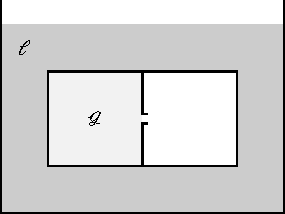
\includegraphics[page=1]{figures/tikz/layouts.pdf}
		\captionof{figure}{Joule的自由膨胀实验}
		\label{fig:Joule free expansion}
	\end{center}
	如\figref{fig:Joule free expansion} 所示,浸在水中的导热容器被活门隔开,一半填充压缩气体,另一半为真空。打开阀门让气体充满整个容器,然后测量过程前后水温的变化,实验测得水温没有发生变化。

	由于气体是向真空膨胀不受外界阻力,$W=0$;水温不变即$Q=0$,继而气体的内能不变,实验结果等价于$(\p T/\p V)_U=0$,
	利用式\eqref{eq:XY*YZ*ZX=-1},可得
	\[
		\pu[T]UV=-\pu[V]UT\pu[U]TV=0.
	\]
	说明气体的内能与体积无关,称为Joule定律。
	\footnote{
		由于水的比热容$\gg$气体的比热容,水的温度变化不易测量,Joule的实验结果并不可靠。
		1852年,Joule和Thomson设计了一个节流膨胀实验来观察实际气体在膨胀时所发生的温度变化,表明实际气体的内能与体积有关。
		尽管如此,Joule定律在低压极限下仍然适用。
		% 我们把严格遵循Boyle定律、Avogadro定律和Joule定律的气体称为理想气体。
	}
\end{example}

\begin{example}
	{理想气体的内能和比热}{ideal gas U and C}
	理想气体遵循Joule定律,$U=U(T)$,可以将等容热容写成导数:
	\begin{equation}
		\label{eq:C_V->U}
		C_V=\dv UT\implies U=\int_{T_0}^TC_V\d T+U_0.
	\end{equation}
	在一定温度范围内,理想气体的等容摩尔热容$C_V/n=cR$为常数,则
	\begin{equation}
		U=cnRT.
	\end{equation}
	其中$c$与理想气体粒子的自由度有关。

	利用\eqref{eq:XY->XY+XW*WY},等容热容和等压热容的差
	\begin{align}
		\notag
		C_p-C_V&=\pu[p]UT+p\pu[p]VT-\pu[V]UT\\
		\notag
		&=\cancel{\pu[V]UT}+\pu[T]UV\pu[p]VT+p\pu[p]VT-\cancel{\pu[V]UT}\\
		&=\biggfkh{\pu[T]UV+p}\pu[p]VT\\
		&=(0+p)\cdot\frac{nR}p=nR.
	\end{align}
	定义热容比
	\begin{equation}
		\gamma:=\frac{C_p}{C_V}=\frac{c+1}{c}.
	\end{equation}
	% 由此便可将$C_p,C_V$用$nR,\gamma$表示出来。
\end{example}

\begin{example}
	{理想气体的四种过程}{}
	理想气体有等容(isochoric, $\d V\equiv 0$)、等压(isobaric, $\d p\equiv 0$)、等温(isothermal, $\d T\equiv 0$)和绝热(adiabatic, $\vd Q\equiv 0$)等不同准静态过程。
	% 对于前三个过程,可简单利用\eqref{eq:pV=nRT}得到关系。
	不同过程在$p\vs V$图中对应的路径如\figref{fig:ideal p-V} 所示,
	% 利用
	% \[
	% 	W=-\int_{V_\text A}^{V_\text B}p\d V,
	% \]
	% 计算功$W$。若方便,可用\eqref{eq:C_V->U}计算内能变化$\D U$,再利用\eqref{eq:dU=dW+dQ}计算热$Q=\D U-W$。
	\begin{center}
		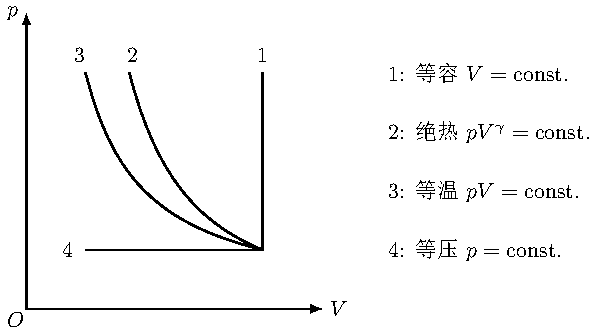
\includegraphics[page=1]{figures/tikz/coordinates.pdf}
		\captionof{figure}{理想气体的$p\vs V$图}
		\label{fig:ideal p-V}
	\end{center}
	\tcblower
	下面研究理想气体的绝热过程。
	由于$\vd Q=0$,可得
	\[
		\d U=0+\vd W=-p\d V,
	\]
	另一方面
	\[
		\d U=C_V\d T
	\]
	此外对理想气体状态方程\eqref{eq:pV=nRT}两边求全微分可得
	\[
		p\d V+V\d p=nR\d T=(C_p-C_V)\d T.
	\]
	结合以上三式,消去$\d T$,%并假设$\gamma=\const$,
	\begin{equation}
		\label{eq:adiabatic}
		\gamma p\d V+V\d p=0\implies pV^\gamma=\const.
	\end{equation}
	由于$\gamma>1$,故$p\vs V$图中的绝热线会比等温线下降得更快,如\figref{fig:ideal p-V} 所示。
\end{example}

\section{热力学第二定律:熵}

热力学第一定律指出各种形式的能量在相互转化的过程中必须满足能量守恒定律,并没有限制过程进行的方向。
但在现实中,涉及热现象的过程都具有方向性。

给定一个初态未平衡的孤立系统,经过一段时间的演化会达到平衡态,这个过程未受环境影响,称为自发过程。
自发过程都是具有方向性的,或者说是不可逆的:
孤立系统不可能自发地回到非平衡的状态。
比如热量可以自发地从高温物体传导到低温物体,但其逆过程却不可能自发发生:热量无法自发地从低温物体传到高温物体。

\begin{theorem}
	{热力学第二定律(Clausius表述)}{second law of thermodynamics (Clausius)}
	不可能把热量从低温物体传到高温物体,而不引起其它变化。
\end{theorem}

\begin{corollary}
	热量从低温物体传到高温物体,必须伴随其它变化,例如做功或热量的转移。
\end{corollary}

\begin{definition}
	{可逆过程}{reversible process}
	给定一个过程,若其逆过程可以使系统和外界都回到原来的状态而无其他变化,则称该过程为可逆过程(reversible process)。
\end{definition}

\begin{corollary}
	无摩擦的准静态过程是可逆过程。
	% 与热现象有关的实际过程都是不可逆过程。
\end{corollary}

\subsection{Carnot循环}

\newcommand{\hi}{_{\mathrm{hi}}}
\newcommand{\lo}{_{\mathrm{lo}}}

热机(heat engine)是实现热和功之间转换的一种系统。
1842年,Carnot通过对热机的总结归纳,指出
热机必须工作于两个热源之间。工作物质从高温热源$T\hi$吸取热量,在低温热源$T\lo$放出热量,这样才能获得机械功。

\begin{example}
	{理想气体的Carnot循环}{Carnot cycle of ideal gas}
	以理想气体为工作物质的Carnot热机,工作过程为四个准静态过程的循环:
	\footnote{约定记号:箭头上的量在过程中$\equiv 0$。
	% 可分别代表等容($\d V\equiv 0$)、等压($\d p\equiv 0$)、等温($\d T\equiv 0$)和绝热($\vd Q\equiv 0$)。
	}
	\[
		\text A(V_\text A,T\hi)
		\overset{\d T}\longrightarrow 
		\text B(V_\text B,T\hi)
		\overset{\vd Q}\longrightarrow 
		\text C(V_\text C,T\lo)
		\overset{\d T}\longrightarrow 
		\text D(V_\text D,T\lo)
		\overset{\vd Q}\longrightarrow 
		\text A(V_\text A,T\hi).
	\]
	称为Carnot循环(carnot cycle),如\figref{fig:Carnot cycle} 所示。\footnote{实线只是示意图,虚线才是正确的形状,单靠坐标伸缩是不可能变成实线那么好看的。}
	\begin{center}
		\includegraphics[page=2]{figures/tikz/coordinates.pdf}
		\captionof{figure}{Carnot循环}
		\label{fig:Carnot cycle}
	\end{center}
	下面分析这个循环的过程
	\begin{alignat*}{2}
		\text A\to\text B~&\text{等温膨胀(吸热):} & Q\hi&=nRT\hi\ln\biggkh{\frac{V_\text B}{V_\text A}};\\
		\text B\to\text C~&\text{绝热膨胀(对外做功):} & \frac{V_\text C}{V_\text B}&=\biggkh{\frac{T\hi}{T\lo}}^c;\\
		\text C\to\text D~&\text{等温压缩(放热):} & Q\lo&=nRT\lo\ln\biggkh{\frac{V_\text C}{V_\text D}};\\
		\text D\to\text A~&\text{绝热压缩(外界对气体做功):} & \frac{V_\text D}{V_\text A}&=\biggkh{\frac{T\hi}{T\lo}}^c.
	\end{alignat*}
	整个循环过程完成后,气体回到原来状态,对外所作的净功为
	\begin{equation}
		W=Q\hi-Q\lo=nR(T\hi-T\lo)\ln\biggkh{\frac{V_\text B}{V_\text A}}.
	\end{equation}
	热功转化的效率
	\begin{equation}
		\eta:=\frac W{Q\hi}=1-\frac{T\lo}{T\hi}<1
	\end{equation}
	这是因为热机只把它从高温热源$T\hi$所吸取的热量$Q\hi$的一部分转化为机械功$W$,其余的热量$Q\lo$在低温热源$T\lo$放出去了。
\end{example}

\begin{corollary}
	Carnot循环是可逆过程。
\end{corollary}

\begin{theorem}{热力学第二定律(Kelvin表述)}{second law of thermodynamics (Kelvin)}
	不可能从单一热源吸热,使之完全变成有用功,而不引起其它变化。
\end{theorem}

\begin{corollary}
	两种表述是等价的。
\end{corollary}

\begin{proof}
	考虑Carnot循环,热机从高温热源$T\hi$吸取热量$Q\hi$、向低温热源$T\lo$放出热量$Q\lo$,对外做功$W=Q\hi-Q\lo$。
	如果Clausius表述不成立,则可以将热量$Q\lo$从$T\lo$传到$T\hi$而不引起其它变化。这相当于热机从单一热源$T\hi$吸取热量$Q\hi-Q\lo$,并将其完全转化为有用功$W$,而不引起其它变化,与Kelvin表述矛盾。

	反之,如果Kelvin表述不成立,则可以从单一热源$T\lo$吸取热量$Q\lo$,并将其完全转化为有用功$W=Q\lo$,而不引起其它变化。将此功完全转化为$T\hi$的热量,就相当于热量从$T\lo$传到$T\hi$而没有引起其他变化,这与Clausius表述矛盾。
\end{proof}

\begin{theorem}{Carnot定理}{Carnot's Theorem}
	在相同高、低温热源之间工作的热机的效率
	\begin{equation}
		\eta=1-\frac{Q\lo}{Q\hi}\leq1-\frac{T\lo}{T\hi}.
	\end{equation}
	取等号当且仅当热机是可逆的。
\end{theorem}

\begin{proof}
	假设可逆热机A和热机B工作在各自的循环中,二者均从高温热源$T\hi$吸收热量均为$Q\hi$,对外做功分别为$W,W'$。
	若$\eta_1<\eta_2$,即$W<W'$,则可将A反向工作,这样两个热机联合的循环相当于从低温热源$T\lo$吸收热量$Q=W'-W$,并将其完全转化为功,而不引起其它变化,这与Kelvin表述矛盾。
	因此$\eta_1\geq\eta_2$。
\end{proof}

\begin{corollary}
	可逆热机效率只与热源温度有关,与工作物质无关。
\end{corollary}

\begin{definition}
	{热力学温标}{thermodynamic temperature scale}
	借助Carnot热机,可通过测量热源吸收/放出的热量的比值来确定温度
	\[
		\frac{Q\lo}{Q\hi}=\frac{T\lo}{T\hi}.
	\]
	钦定水
	\footnote{这里需要给出水的严格定义,包括H和O的同位素比例。
	% 定义水的分子式为$\mathrm{H_2O}$,其同位素的成分为
	% \begin{align*}
	% 	n_\mathrm{H^1}:n_\mathrm{H^2}&=1:1.5576\times10^{-4},\\
	% 	n_\mathrm{O^{16}}:n_\mathrm{O^{17}}:n_\mathrm{O^{18}}&=1:3.799\times 10^{-4}:2.0052\times 10^{-3}.
	% \end{align*}
	}
	的三相点温度$T_0=\SI{273.16}{\kelvin}$作为参考温度后,便可完全确定其他物质的温度。
	这种温标不依赖于具体的工作物质,因此是绝对的,称为热力学温标(thermodynamic temperature scale),也称Kelvin温标。
\end{definition}

% \begin{remark}
% 	为了准确测定温度,我们不止需要指定温度的特殊点,还需要指定测温物质和测温属性。例如,单纯利用物体的热膨胀测温,那么水银温度计和酒精温度计将会给出不同的温度结果。而热力学温标与测温物质无关的特性,使得它在物理中被广泛运用。
% \end{remark}

\subsection{熵}

\begin{theorem}{Clausius不等式}{Clausius inequality}
	在循环过程中,系统吸收的热量$\vd Q$及温度$T$满足
	\begin{equation}
		\oint\frac{\vd Q}T\leqslant 0.
	\end{equation}
	当且仅当为可逆循环时取等号。
\end{theorem}

\begin{proof}
	考虑一个热机循环,热机从高温热源$T\hi$吸收热量$Q\hi$,向低温热源$T\lo$吸收热量$Q\lo$ (即放出热量$-Q\lo$)。
	由Carnot定理可知
	\[
		\eta=1-\frac{-Q\lo}{Q\hi}\leq1-\frac{T\lo}{T\hi}
		\implies
		\frac{Q\hi}{T\hi}+\frac{Q\lo}{T\lo}\leq 0.
	\]
	当且仅当热机可逆时取等号。
	考虑若干个热机循环叠加成的热力学循环,从热源$T_1,\ldots,T_k$吸收热量$Q_1,\ldots,Q_k$,则
	\[
		\sum_{i=1}^k\frac{Q_i}{T_i}\leq 0,
	\]
	取等号当且仅当所有循环都是可逆的。任意热力学循环都可作为这种叠加的极限情况,对应地将求和改为积分即可。
\end{proof}

\begin{corollary}
	考虑任意经过$\text A\to\text B$的两个可逆过程$\text R,\text R'$,并记$\text R'$的逆过程为$-\text R'$,则$\text R+(-\text R')\equiv\text R-\text R'$构成一个可逆循环,由Clausius不等式:
	\[
		\oint_{\text R-\text R'}\frac{\vd Q}T=\int_\text R\frac{\vd Q}T+\int_{-\text R'}\frac{\vd Q}T=0\implies
		\int_\text R\frac{\vd Q}T=\int_{\text R'}\frac{\vd Q}T,
	\]
	因此对于经过$\text A\to\text B$的任意可逆过程,$\vd Q/T$的积分都是相同的,与过程的具体路径无关,由此可写成微分的形式。
\end{corollary}

\begin{definition}
	{熵}{entropy}
	对于可逆过程,可定义微分
	\begin{equation}
		\label{eq:dS=dQ/T}
		\d S:=\frac{\vd Q}T.
	\end{equation}
	称$S$为熵(entropy)。
\end{definition}

\begin{corollary}
	考虑R为不可逆过程,由Clausius不等式可得,不可逆过程$\d S>\vd Q/T$。
\end{corollary}

\begin{theorem}
	{熵增加原理}{principle of entropy increase}
	在绝热条件下,系统在可逆过程中$\D S=0$,不可逆过程$\D S>0$,熵不可能减少。
\end{theorem}

\begin{corollary}
	平衡态时熵取最大值,继而熵函数$S=S(U,V)$应该是严格上凸的。
	% \[
	% 	\pv[2]SU\pv[2]SV>\biggkh{\pw SUV}^2>0.
	% \]
\end{corollary}

% 熵是热运动混乱程度的量度。

% \begin{example}{熵的计算}{Calculating Entropy}
% 	将质量相同而温度分别为$T_1$和$T_2$的两杯水在等压下绝热的混合,求熵变。

% 	终态温度$T=(T_1+T_2)/2$,第一杯水的熵变为
% 	\[
% 		\D S_1=\int_{T_1}^T\frac{C_p\d T}T=C_p\ln\frac{T_1+T_2}{2T_1},
% 	\]
% 	第二杯水的熵变$\D S_2$同理可求,
% 	总熵增
% 	\[
% 		\D S_1+\D S_2=C_p\ln\frac{(T_1+T_2)^2}{4T_1T_2}\geqslant 0.
% 	\]
% 	取等号当且仅当$T_1=T_2$。
% \end{example}

\begin{theorem}
	{热力学基本微分方程}{}
	在可逆过程中,由热力学第一定律\eqref{eq:dU=dW+dQ}和熵的定义\eqref{eq:dS=dQ/T},可将$\d U$写成全微分形式:
	\begin{equation}
		\label{eq:dU=TdS-pdV}
		\d U=T\d S-p\d V.
	\end{equation}
\end{theorem}

\begin{corollary}
	根据全微分与偏导数的关系,温度和压强可以写成偏导形式:
	\begin{subequations}
		\begin{align}
			T&=\pu[V]US,\\
			p&=-\pu[S]UV.
		\end{align}
	\end{subequations}
	在熵表象下,考虑$S$的全微分,可由\eqref{eq:dU=TdS-pdV}直接得出
	\begin{equation}
		\d S=\frac1T\d U+\frac pT\d V.
	\end{equation}
	以及$S$的偏导数
	\begin{subequations}
		\begin{align}
			\pu[V]SU&=\frac1T,\\
			\pu[U]SV&=\frac pT.
		\end{align}
	\end{subequations}
\end{corollary}

% \begin{theorem}
% 	{熵函数的凹凸性}{concavity of entropy function}
% 	$S=S(U,V)$是严格上凸的(strictly concave)。
% \end{theorem}

% \begin{proof}
% 	固定$V$,对于内能为$2U$的系统,其两个子系统内能$U_\pm=U\pm\D U$。不均匀的子系统熵更低,即
% 	\[
% 		S(U+\D U)+S(U-\D U)<S(2U)=2S(U)
% 		\implies\pv[2]SU<0,
% 	\]
% \end{proof}

\begin{corollary}
	由$S$上凸,
	$1/T=(\p S/\p U)_V$是$U$的减函数,因此系统温度越高,内能越大。
\end{corollary}

\begin{example}
	{温度$T$的热力学意义}{}
	封闭系统由导热壁($V$恒定,$U$可变)隔开,子系统的内能满足
	\[
		U_1+U_2=\const\implies\d U_1=-\d U_2.
	\]
	平衡时熵达到极值,有
	\[
		\d S=\d S_1+\d S_2=\pv{S_1}{U_1}\d U_1+\pv{S_2}{U_2}\d U_2=\biggkh{\frac1{T_1}-\frac1{T_2}}\d U_1=0\implies T_1=T_2.
	\]
	故平衡时子系统温度相等;
	若初始时温度$T_1^0<T_2^0$,平衡温度$T$。由能量守恒,应有
	\[
		T_1^0<T<T_2^0,
	\]
	这说明\textit{热量总是从高温流向低温},这符合现实中温度的特性。
\end{example}

\begin{example}
	{压强$p$的热力学意义}{}
	系统由导热
	% \footnote{熵表象下的绝热活塞讨论比较微妙。}
	活塞($U,V$可变)隔开,平衡时
	\[
		\d S=\d S_1+\d S_2=\biggkh{\frac1{T_1}-\frac1{T_2}}\d U_1+\biggkh{\frac{p_1}{T_1}-\frac{p_2}{T_2}}\d V_1=0\implies T_1=T_2,p_1=p_2
	\]
	平衡时压强相等。同理,可以进而推出\textit{压强大的一侧会推动活塞}。
	% 换成导热半透膜($V$恒定,$U,N$可变)隔开,可以得到$T_1=T_2,N_1=N_2$的结论,说明\textit{物质总是由化学势高流向化学势低的一边}。
\end{example}

\begin{example}
	{理想气体的熵}{entropy of ideal gas}
	考虑理想气体的微分
	\[
		\d S=\frac1T\d U+\frac pT\d V=\frac{C_V}T\d T+\frac{nR}V\d V.
	\]
	采用$C_V=cnR$,可得
	\[
		\d S=nR\biggkh{c\frac{\d T}T+\frac{\d V}V}\implies S=nR\ln\biggfkh{\biggkh{\frac{T}{T_0}}^c\biggkh{\frac{V}{V_0}}}+S_0.
	\]
	因此,对于可逆绝热过程,$\d S=0$,从而$T^cV=\const$。	
\end{example}

\paragraph{用过程求熵}

因为熵的变化只与始末态有关,我们可以用一个连接初态和末态的过程测量熵的变化,%我们可以让这个过程有比较良好的性质:各子系统无限接近平衡。由于
%$$\d U=\vd Q+\vd W+\vd W_r.$$
%其中$\vd Q$为传热,$\vd W=-P\d V$为功,$\vd W_r$为耗散,则熵的变化
%$$\d S=\frac1T\d U+\frac PT\d V=\frac{\vd Q+\vd W_r}T.$$
%因为在准静态过程中,\textit{只有热和耗散导致了熵的增加}。我们可以构造特定的过程,
这样只需要知道此\textit{过程中的状态方程}就可以求出熵变了。

\begin{example}
	{理想气体自由膨胀}{}
	理想气体从$V$自由(绝热)膨胀到$\lambda V$,其熵增为
	\[
		\D S=nR\ln\lambda.
	\]
	显然$\D S>0$,然而实际上$Q\equiv 0$。因此自由膨胀是非准静态的,更不可逆。
	\tcblower
	自由膨胀过程是$\text A\to\text C$的等温过程(但这一过程$\vd W=\vd Q=0$,并非准静态过程),
	为了求其熵变,可以构造这样一个先$\text A\to\text B$绝热,后$\text B\to\text C$等容的过程
	\[
		\text A(V,p_\text A)\overset{\vd Q}\longrightarrow\text B(\lambda V,p_\text B)\overset{\d V}\longrightarrow\text C(\lambda V,p_\text C).
	\]
	\begin{center}
		\includegraphics[page=4]{figures/tikz/coordinates.pdf}		
		\captionof{figure}{$p\vs V$图像中的过程}
	\end{center}
	$\text A\to\text B$绝热,$T^cV=\const.$因此$T_\text A^c=\lambda T_\text B^c.$\\[1ex]
	$\text B\to\text C$等容,$\vd Q=\d U=cnR\d T$,故 
	\[
		\D S=\int_\text B^\text C\frac{\vd Q}T=cnR\int_\text B^\text A\frac{\d T}T=nR\ln\lambda.
	\]
	与$\text A\to\text C$等温过程的熵变相同。
\end{example}


\section{热力学第三定律:绝对零度}

相较于前几个基本定律,
热力学第三定律的出现得非常晚。
本节适合在学习完\chapref{chap:simple system}后阅读。

\subsectionstar{低温的获得}

% 物理中有各种能量尺度。 在一定的温度下,相应能量尺度(∼ kBT)的现象会显现出来。
为了探索更低能量尺度上的物理,人们需要越来越低的温度。最终人们发现气体是最容易降温的一种物质。所以早期获得低温的历史基本上是液化气体的历史。其他系统的降温只要与液化气体接触就可以实现。气体液化是十九世纪末二十世纪初的一项重要科学成就。在1877、1883、1898和1908年氧气、氮气、氢气和氦气分别被液化。
% 液化气体的关键在于降低气体分子的动能,这样由于分子间的吸引力,可将气体液化。降低动能有各种不同的方法,但基本上都是使气体绝热膨胀。实现绝热膨胀的方法不同,对温度的改变也不同。气体液化后再降温会比较困难,但液化后的气体有很大的潜热,可用于保持恒温。

\begin{example}
	{Joule-Thomson节流膨胀实验}{}
	% 鉴于1843年,Joule的自由膨胀实验不够精确,1852年Joule和Thomson设计了一个节流膨胀实验来观察实际气体在膨胀时所发生的温度变化。
	如\figref{fig:Joule throttle expansion} 所示,在一个圆形绝热筒的中部,置有一个刚性的多孔塞,
	实验时,将压力和温度恒定为$p_1$和$T_1$的某种气体,连续地压过多孔塞,使气体在多孔塞右边的压力恒定为$p_2$,且$p_1>p_2$。
	\footnote{由于多孔塞的孔很小,气体只能缓慢地从左侧进入右侧,并且可保持左室$p_1$部分和右室低压$p_2$的部分压力恒定不变。这种维持一定压力差的绝热膨胀过程叫做节流膨胀。}
	\begin{center}
		\includegraphics[page=2]{figures/tikz/layouts.pdf}
		\captionof{figure}{Joule-Thomson节流膨胀实验}
		\label{fig:Joule throttle expansion}
	\end{center}
	将1中所有的气体推到2后,
	\[
		\D U=U_2-U_1=-p_2V_2+p_1V_1+0,
	\]
	即
	\[
		U_1+p_1V_1=U_2+p_2V_2\implies H_1=H_2.
	\]
	因此节流膨胀过程焓变$\D H=0$。
\end{example}

\begin{remark}
	真实的节流过程不是等焓过程,甚至都不是准静态过程。但是之所以可以用等焓来讨论,是因为初、末态的焓经过节流过程不变。
\end{remark}

\begin{theorem}
	{Joule-Thomson效应}{}
	由\eqref{eq:XY->XW/YW}和Maxwell关系\eqref{eq:Maxwell relation G}:
	\begin{equation}
		\pu[H]Tp=-\division{\pu[T]Hp}{\pu[p]HT}=-\frac1{C_p}\biggfkh{T\pu[T]Sp+V}=\frac{V(T\alpha-1)}{C_p}.
	\end{equation}
	当$T\alpha>1$时,高压向低压的节流过程可以降低温度。
\end{theorem}
\begin{remark}
	理想气体$T\alpha=1$,不能通过节流过程改变温度。
	但实际气体在一定条件下会有相当大的Joule-Thomson效应,Onnes就是利用这种效应首次将He液化。
\end{remark}

% 若要获得尽可能低的温度,一种方法是让气体绝热膨胀;另一种是自由膨胀(所幸现实中的气体并不理想)。
\begin{example}
	{通过van der Waals气体实现降温}{}
	考虑van der Waals气体,其热膨胀系数
	\[
		\alpha=\frac1v\pu[p]vT=\fkh{\frac{Tv}{v-b}-\frac{2a(v-b)}{Rv^2}}^{-1}
	\]
	为了使$\alpha T>1$,应有
	\[
		T>\frac{2a}{bR}\biggkh{\frac{v-b}v}^2,
	\]
	转化为压强$p$和温度$T$的关系:
	\[
		p<\frac a{b^2}\biggkh{1-\sqrt{\frac{RbT}{2a}}}\biggkh{3\sqrt{\frac{RbT}{2a}}-1}.
	\]
	%,\quad  p=\frac{RT}{v-b}-\frac a{v^2}\\%\frac bv>1-\sqrt{\frac{bRT}{2a}}
	\begin{center}
		\includegraphics[page=5]{figures/tikz/coordinates.pdf}
		\captionof{figure}{van der Waals气体实现降温的条件}
	\end{center}
\end{example}

\subsection{Nernst定理}

1906年,Nernst在研究各种化学反应在低温下的性质时,由于
\[
	\frac{\D G-\D H}T=-\D S
	% \implies\lim_{T\to 0}\frac{\D G}T-\lim_{T\to 0}\frac{\D H}T=-\lim_{T\to 0}(\D S)_T.
\]
实验说明:低温下$\D H$相当接近$\D G$,因此可以期待$\D H,\D G$在$T=0$处具有相同的斜率。

\begin{theorem}
	{Nernst定理}{Nernst theorem}
	温度$T\to 0$时,等温过程的熵变$(\D S)_T\to 0$:
	\begin{equation}
		\lim_{T\to 0}(\D S)_T=0.
	\end{equation}
\end{theorem}

\begin{corollary}
	温度$T\to 0$时,同一物质的一切平衡态都具有相同的熵,通常直接取为0,即
	\begin{equation}
		\lim_{T\to 0}S(T,p)=S(0,p):=0.
	\end{equation}
\end{corollary}

\begin{theorem}
	{热力学第三定律}{third law of thermodynamics}
	不可能通过有限的步骤使一个物体冷却到热力学温度的零度。
\end{theorem}

